\section{分析 wa}

% \begin{frame}{分析 wa}
%     \centering
%     \Large \textbf{分析 wa}
% \end{frame}

\begin{frame}{代码中处理 wa 存在的问题}
	\begin{itemize}
		\item 代码中的 WA 处理方式存在问题,它没有对 WA 返回的结果进行有效处理。
		      \bigskip
		\item 大量无关信息被直接传递给大模型,可能会影响大模型的推理。
		      % \item 
		      %  \item 
	\end{itemize}
\end{frame}

\begin{frame}{WA 返回信息示例}
	\textbf{例如}: 对于计算 $ 2*17-1 $ 时,wa 的返回结果如下:
	% \centering
	\begin{figure}
		
\includegraphics[width=0.5\textwidth]{./pic/2.png}
	\end{figure}

	实际上,返回结果中只有 \texttt{@inputstring'} 和 \texttt{'plaintext'} 是有用的信息。
\end{frame}

\begin{frame}{调用 wa 的常见错误}
	\begin{itemize}
		\item \textbf{生成的查询过于复杂}: 不符合 wa 语法规范,无法获得答案。
		      \begin{itemize}
			      \item 例如,对于查询语句:
			            \texttt{Calculate the distances PQ, QR, PR; check which sides form a right angle; use ((1)/(2)) × base × height to find the area of $\triangle$ PQR.}
		      \end{itemize}
		      \pause
		      \bigskip
		\item \textbf{混杂自然语言}: 生成了正确的 wa 查询语句,但是混杂在自然语言中。
		      \begin{itemize}
			      \item 例如,对于查询语句:
			            \texttt{Find the minimum x greater than 10 such that PrimeQ[x + 7] \&\& PrimeQ[x + 13] \&\& PrimeQ[x + 15].}
			      \item wa 返回结果:
			            \texttt{'@success': False, Did you mean: PrimeQ[x + 7] \&\& PrimeQ[x + 13] \&\& PrimeQ[x + 15] ?}
			      \item  如果按照 wa 的提示,把\texttt{PrimeQ[x + 7] \&\& PrimeQ[x + 13] \&\& PrimeQ[x + 15]} 作为查询语句再次调用 wa ,wa 是可以理解的,但这和我们的问题没有关联。
			      \item 如何把 \texttt{Find the minimum x greater than 10 such that PrimeQ[x + 7] \&\& PrimeQ[x + 13] \&\& PrimeQ[x + 15].} 转换为一个有效的 wa 查询语句?这似乎非常困难。
		      \end{itemize}
	\end{itemize}
\end{frame}

\begin{frame}{wa 的纠错方式}
	\begin{itemize}
		\item   代码中有纠错的方式,如果返回结果中\texttt{@success}为false,则再生成新的查询并调用 wa ,最多尝试三次。
		      \pause
		      %  \bigskip
		\item 但是,三次都失败的概率并不低。
		      \begin{itemize}
			      \item 对于 qwen2.5:32b-instruct-fp16,100个测试样例有11个样例出现3次调用wa均失败的情况。
			      \item 对于 4o-mini,100个测试样例有12个样例出现3次调用wa均失败的情况。
		      \end{itemize}
		      \pause
		      % \bigskip
		\item 增加最大尝试次数对于提高正确率帮助很小,并且显著增加推理时间。
		      \pause
		      % \bigskip
		\item 性能较差的模型还有其他问题,例如,使用 qwen2.5:7b-instruct-fp16,发现 7b 模型有很多次出现生成的内容没有 \texttt{Final Query:} 字符串,导致提取失败而多次尝试的情况(4omini和qwen2.5:32b-instruct-fp16没有观察到),并且有四例十次最终没有生成 wa 查询语句的情况(不是生成了错误的查询,是 llm 生成的内容没有相应的关键词而无法提取出查询)
	\end{itemize}
	% \pause
	% \bigskip
	
	
	
\end{frame}
\begin{frame}
	\begin{itemize}
		\item 对于性能较差的模型来说,正则匹配或者关键词提取可能不是一个很好的方式,可以考虑结构化输出的方式。
		\pause
		\bigskip
		\item 例如,查阅 qwen api 文档,发现结构化输出功能支持qwen2.5系列所有模型(除了math与coder模型)。
	\end{itemize}
	
	
\end{frame}
\begin{frame}
	\begin{figure}
		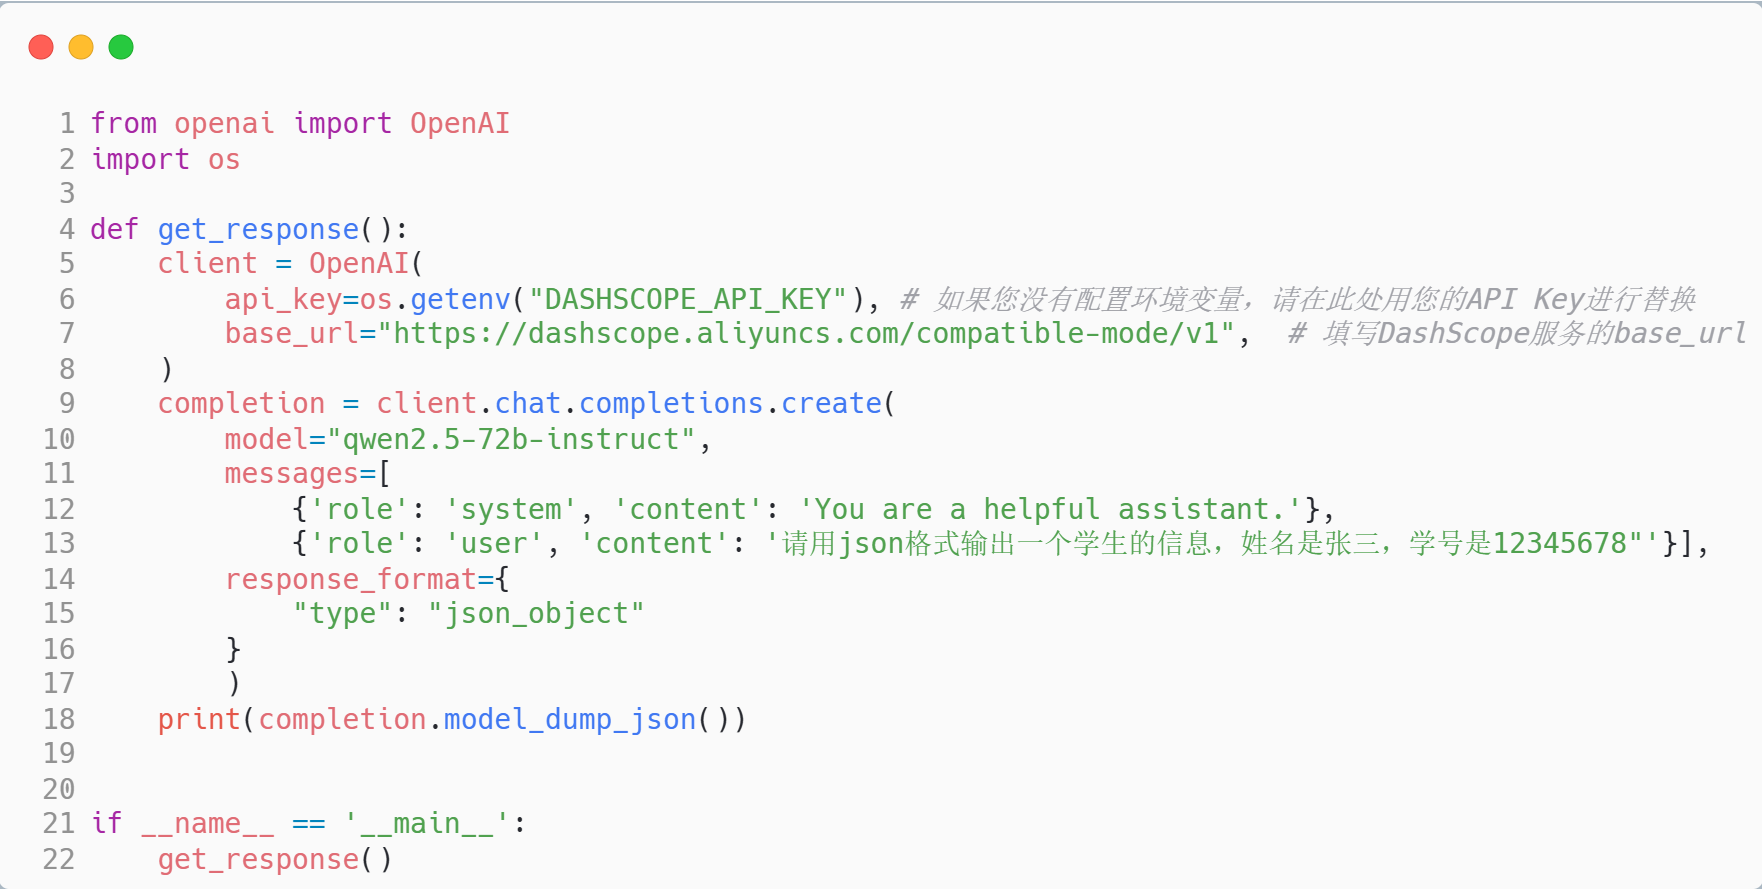
\includegraphics[width=0.8\textwidth]{./pic/3.png}
		\caption{qwen api 文档结构化输出示例请求}
	\end{figure}
\end{frame}

\begin{frame}
	\begin{figure}
		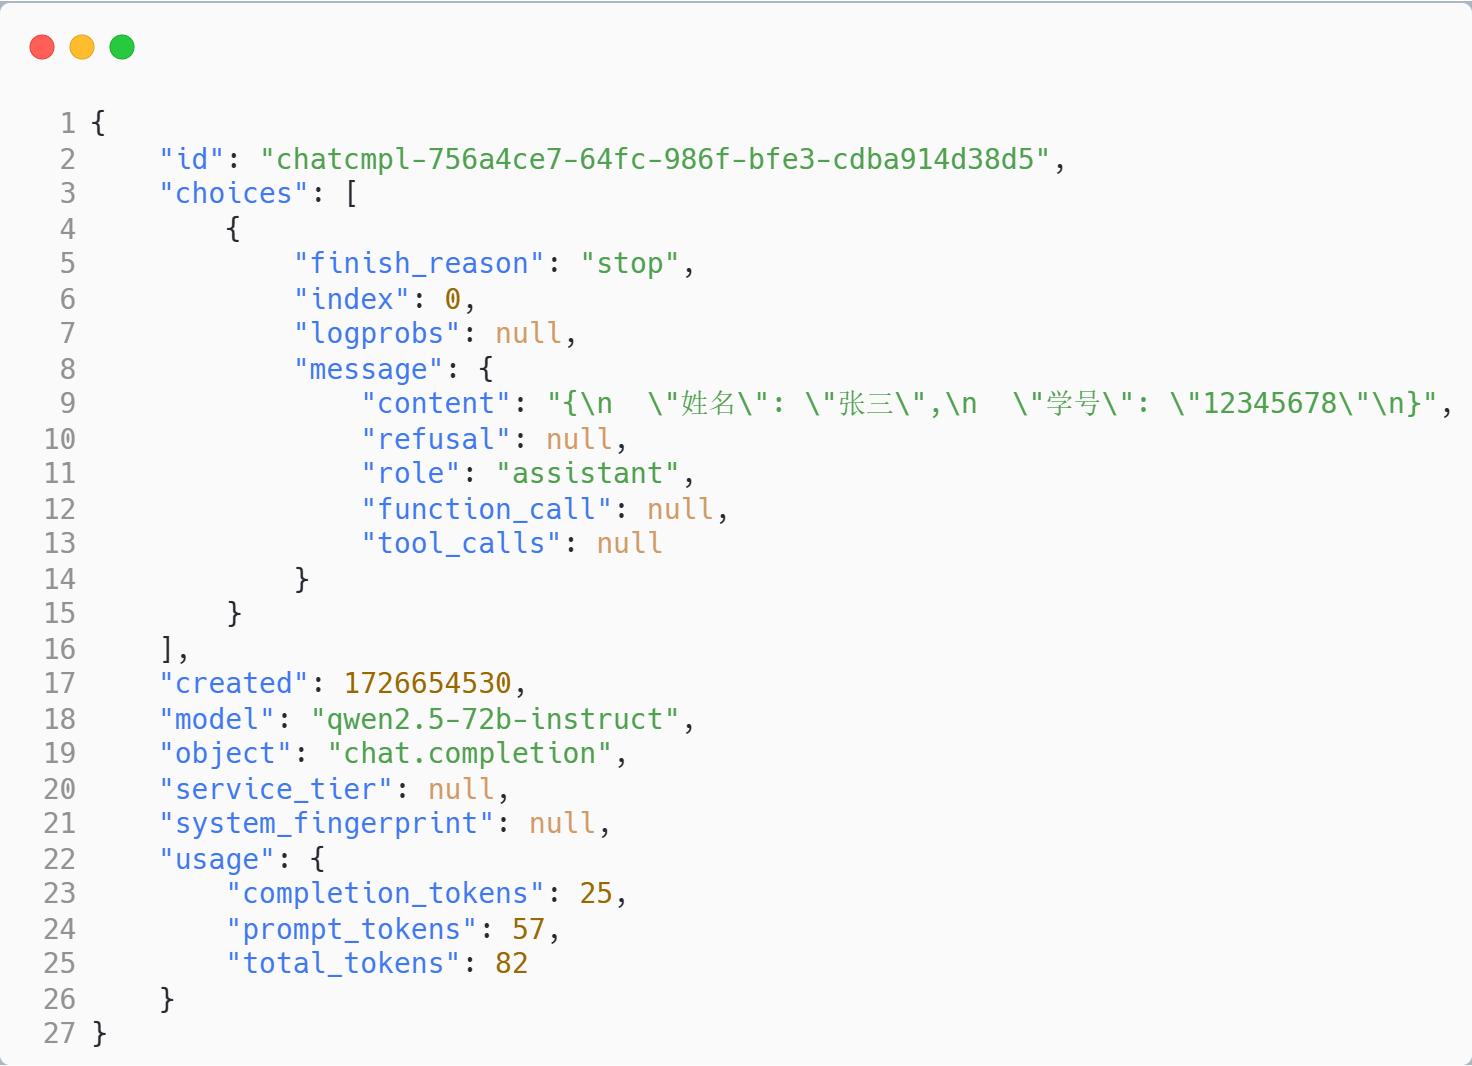
\includegraphics[width=0.6\textwidth]{./pic/4.png}
		\caption{qwen api 文档结构化输出示例响应}
	\end{figure}
\end{frame}

\begin{frame}
	\textbf{问:有什么方式增加生成正确查询的概率?}
	\begin{itemize}
		\item 在 prompt 中加入一些合法的 wa 查询作为 few-shot 是否可行?大概需要多少条才能有效提升生成正确查询的概率?
		\bigskip
		\item 如何分解问题,多次调用 wa?
		\bigskip
		\item 如何结合 CoT 、ToT 等方式?
		\pause
		\bigskip
		\item 对于类似于\texttt{Find the minimum x greater than 10 such that PrimeQ[x + 7] \&\& PrimeQ[x + 13] \&\& PrimeQ[x + 15].} 这种很难转化为 wa 查询的问题,是否可以结合 python 程序去解决?什么样的问题适合用 python 程序解决?什么样的问题适合用 wa 解决?如果 wa 和 python 都使用,对于一个具体的问题,LLM 如何决策选择哪一种工具?更复杂地,如果一个问题经过分解后,有一部分适合用 wa 解决,有一部分适合用 python 解决,LLM 如何决策?
	\end{itemize}
\end{frame}